\documentclass[xcolor=x11names,compress]{beamer}
%% General document %%%%%%%%%%%%%%%%%%%%%%%%%%%%%%%%%%
\usepackage{graphicx}
\usepackage{tikz}
\usetikzlibrary{decorations.fractals}
%%%%%%%%%%%%%%%%%%%%%%%%%%%%%%%%%%%%%%%%%%%%%%%%%%%%%%
%% Beamer Layout %%%%%%%%%%%%%%%%%%%%%%%%%%%%%%%%%%
\useoutertheme[subsection=false,shadow]{miniframes}
\useinnertheme{default}
\usefonttheme{serif}
\usepackage{palatino}
\usepackage{setspace,textcomp,soul}

\setbeamerfont{title like}{shape=\scshape}
\setbeamerfont{frametitle}{shape=\scshape}
\definecolor{bluUnicam}{RGB}{27,43,74}
\definecolor{redUnicam}{RGB}{219,0,36}
\definecolor{orangeUnicam}{RGB}{234,114,40}
\setbeamercolor*{lower separation line head}{bg=redUnicam} 
\setbeamercolor*{normal text}{fg=bluUnicam,bg=white} 
\setbeamercolor*{alerted text}{fg=red} 
\setbeamercolor*{example text}{fg=black} 
\setbeamercolor*{structure}{fg=orangeUnicam} 
\setbeamercolor*{frametitle}{fg=redUnicam}

\setbeamercolor*{palette tertiary}{fg=orangeUnicam,bg=bluUnicam} 
\setbeamercolor*{palette quaternary}{fg=black,bg=black!10} 

%%%%%%%%%%%%%%%%%%%%%%%%%%%%%%%%%%%%%%%%%%%%%%%%%%
%% Author data and Logo %%%%%%%%%%%%%%%%%%%%%%%%%%
\subtitle{Current Work Status}
\author[shortname]{
    {\textbf{Francesco Moschella\\}}
    \fontsize{8pt}{10}\selectfont{francesco.moschella@studenti.unicam.it}
}

\date{
	\begin{figure}[htpb!]
    	\centering
        
\includegraphics[width=0.15\textwidth]{figures/logo}
        \hspace*{0.5cm}
        
\includegraphics[width=0.20\textwidth]{figures/ru-logo}
    \end{figure}
    %\today
}

\newcommand{\red}[1]{{\color{red}#1}}

\begin{document}
%%%%%%%%%%%%%%%%%%%%%%%%%%%%%%%%%%%%%%%%%%%%%%%%%%%%%%
%%%%%%%%%%%%%%%%%%%%%%%%%%%%%%%%%%%%%%%%%%%%%%%%%%%%%%
\section{\scshape}
\begin{frame}
    \begin{center}
        \title{\color{redUnicam}{Game Control using EEG Motor Imagery}}
        \titlepage
    \end{center}
\end{frame}

\begin{frame}{Outline}
    \tableofcontents
\end{frame}
%%%%%%%%%%%%%%%%%%%%%%%%%%%%%%%%%%%%%%%%%%%%%%%%%%%%%%
%%%%%%%%%%%%%%%%%%%%%%%%%%%%%%%%%%%%%%%%%%%%%%%%%%%%%%
\section{Introduction}
\begin{frame}{Introduction}
\begin{itemize}
    \item \textbf{Research Question:} Is it possible to perform Real-Time Motor Imagery (MI) Classification?
    \item \textbf{Objective 1:} Develop a Real-Time Motor Imagery Classification System
    \item \textbf{Objective 2:} Develop a Dataset Augmentation Technique to Test the System
    \item \textbf{Objective 3:} Develop a Virtual Environment where the User will be able to Control a Virtual agent using EEG MI Signals
\end{itemize}
\end{frame}
\section{Related Works}
\begin{frame}{Related Works}
    \begin{minipage}[c]{0.65\textwidth}
        \begin{itemize}
            \item EEG MI Classifier
            \item Dataset Augmentation
            \item User Game Feel and Experience
            \item EEG MI Uses in Real Case-Scenarios
        \end{itemize}
    \end{minipage}
    \begin{minipage}[c]{0.33\textwidth}
        \vspace*{-.5cm}
        \hspace*{-.7cm}
        \begin{tikzpicture}
            \node (page1) [yshift=4.5cm, xshift=-.5cm, rotate=30] {
                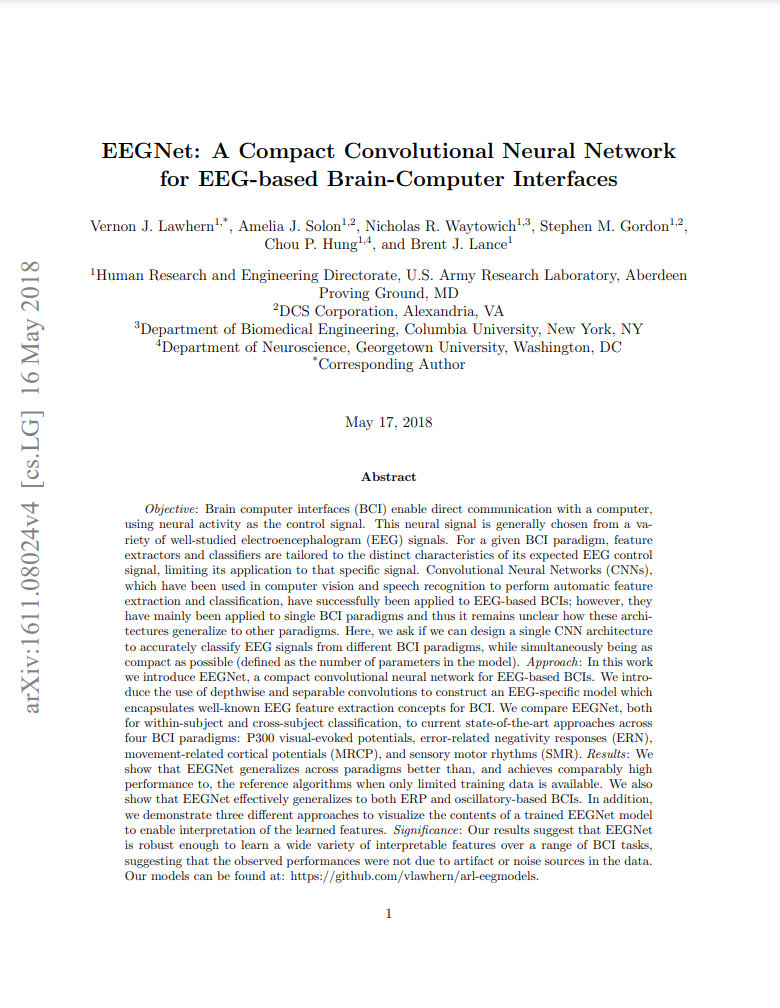
\includegraphics[width=0.4\textwidth]{figures/literature/classifier/EEGNet_paper}
            };
            \node (page2) [yshift=4.5cm, xshift=.5cm, rotate=-30] {
                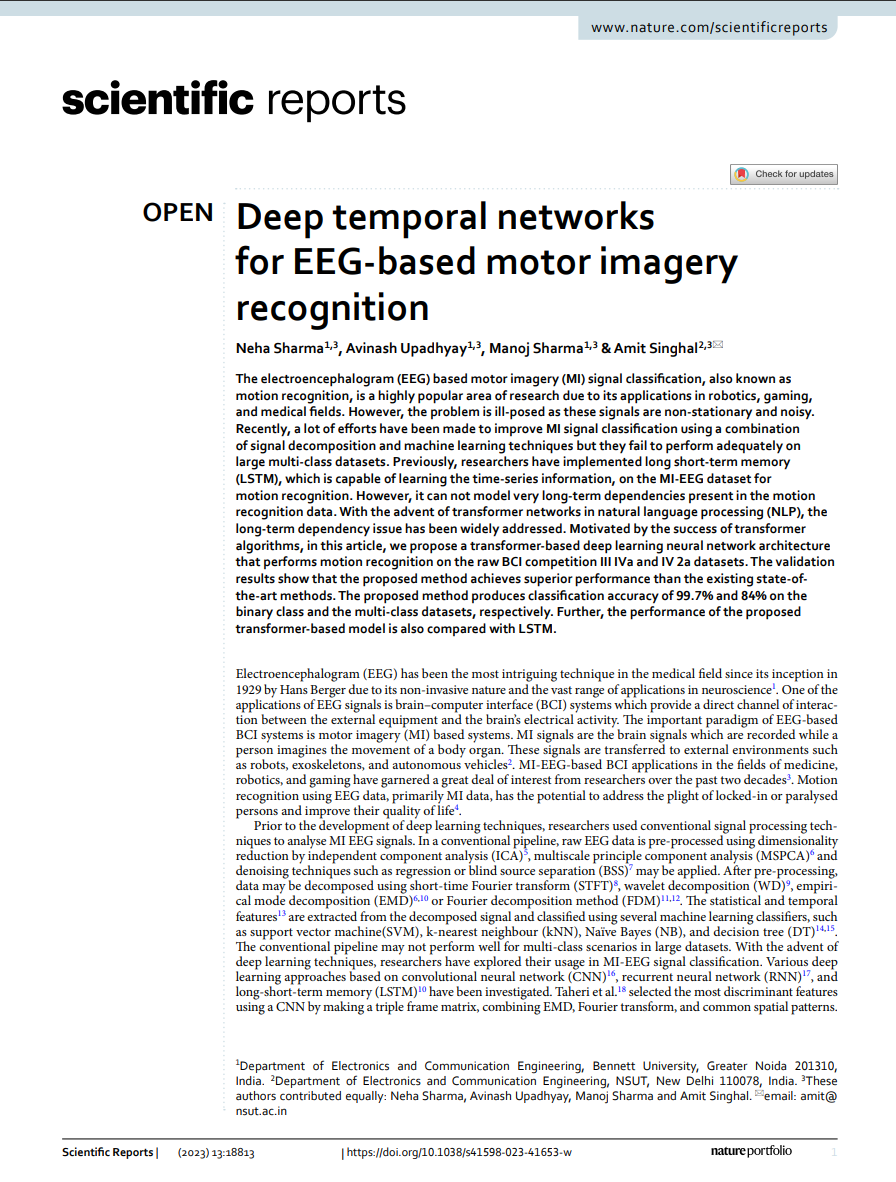
\includegraphics[width=0.4\textwidth]{figures/literature/classifier/LSTM_Transformer_paper}
            };
            %
            \node (page3) [yshift=3cm, xshift=-.5cm, rotate=30] {
                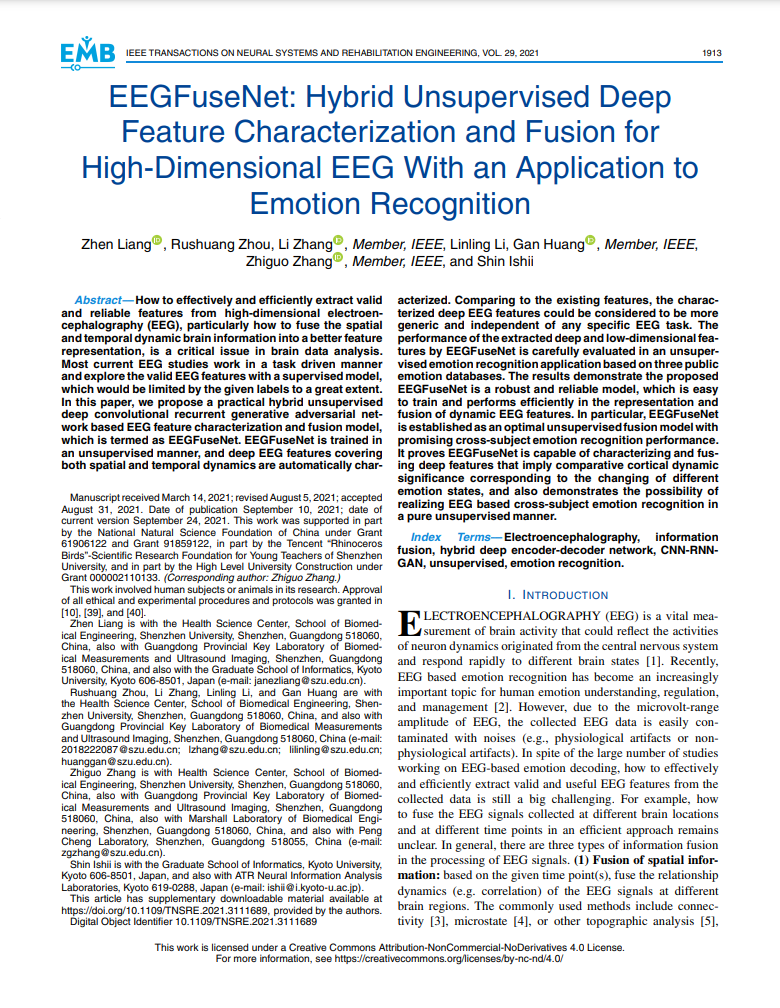
\includegraphics[width=0.4\textwidth]{figures/literature/augmentation/EEGFuseNet_paper}
            };
            \node (page4) [yshift=3cm, xshift=.5cm, rotate=-30] {
                
\includegraphics[width=0.4\textwidth]{figures/literature/augmentation/NoiseInjection_paper}
            };
            %
            \node (page5) [yshift=1.5cm, xshift=-.5cm, rotate=30] {
                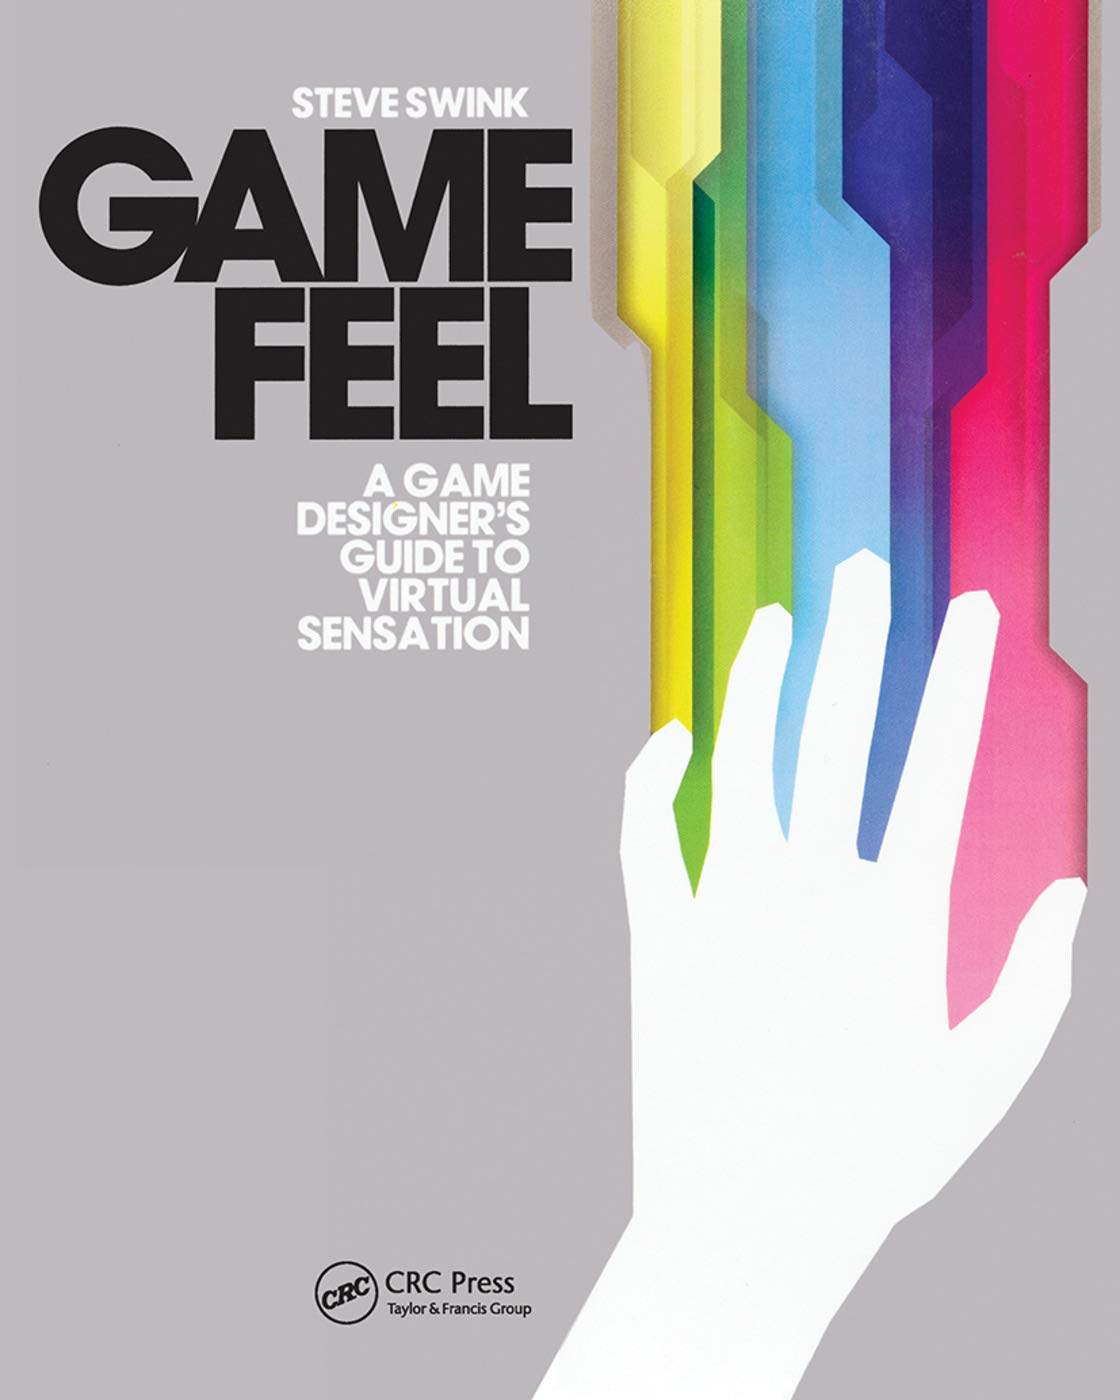
\includegraphics[width=0.4\textwidth]{figures/literature/gamefeel/GameFeel_book}
            };
            \node (page6) [yshift=1.5cm, xshift=.5cm, rotate=-30] {
                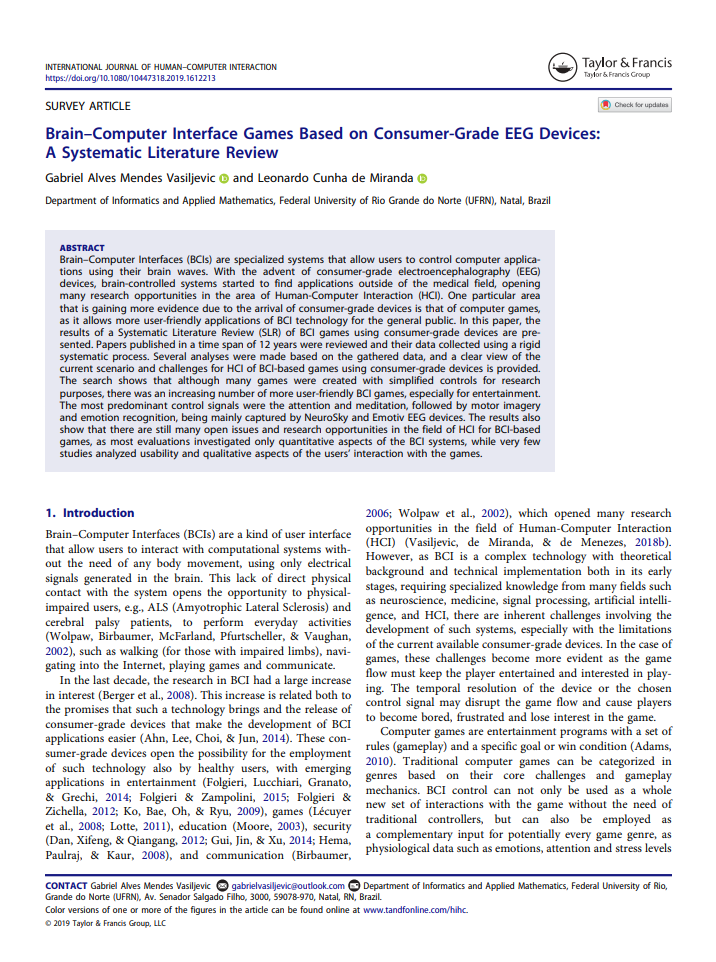
\includegraphics[width=0.4\textwidth]{figures/literature/gamefeel/BCI_Game_paper}
            };
            %
            
            \node (page9) [yshift=0cm, xshift=-1.5cm, rotate=30] {
                
\includegraphics[width=0.4\textwidth]{figures/literature/realcase/WheelchairControl_paper}
            };
            \node (page11) [yshift=0cm, xshift=1.5cm, rotate=-30] {
                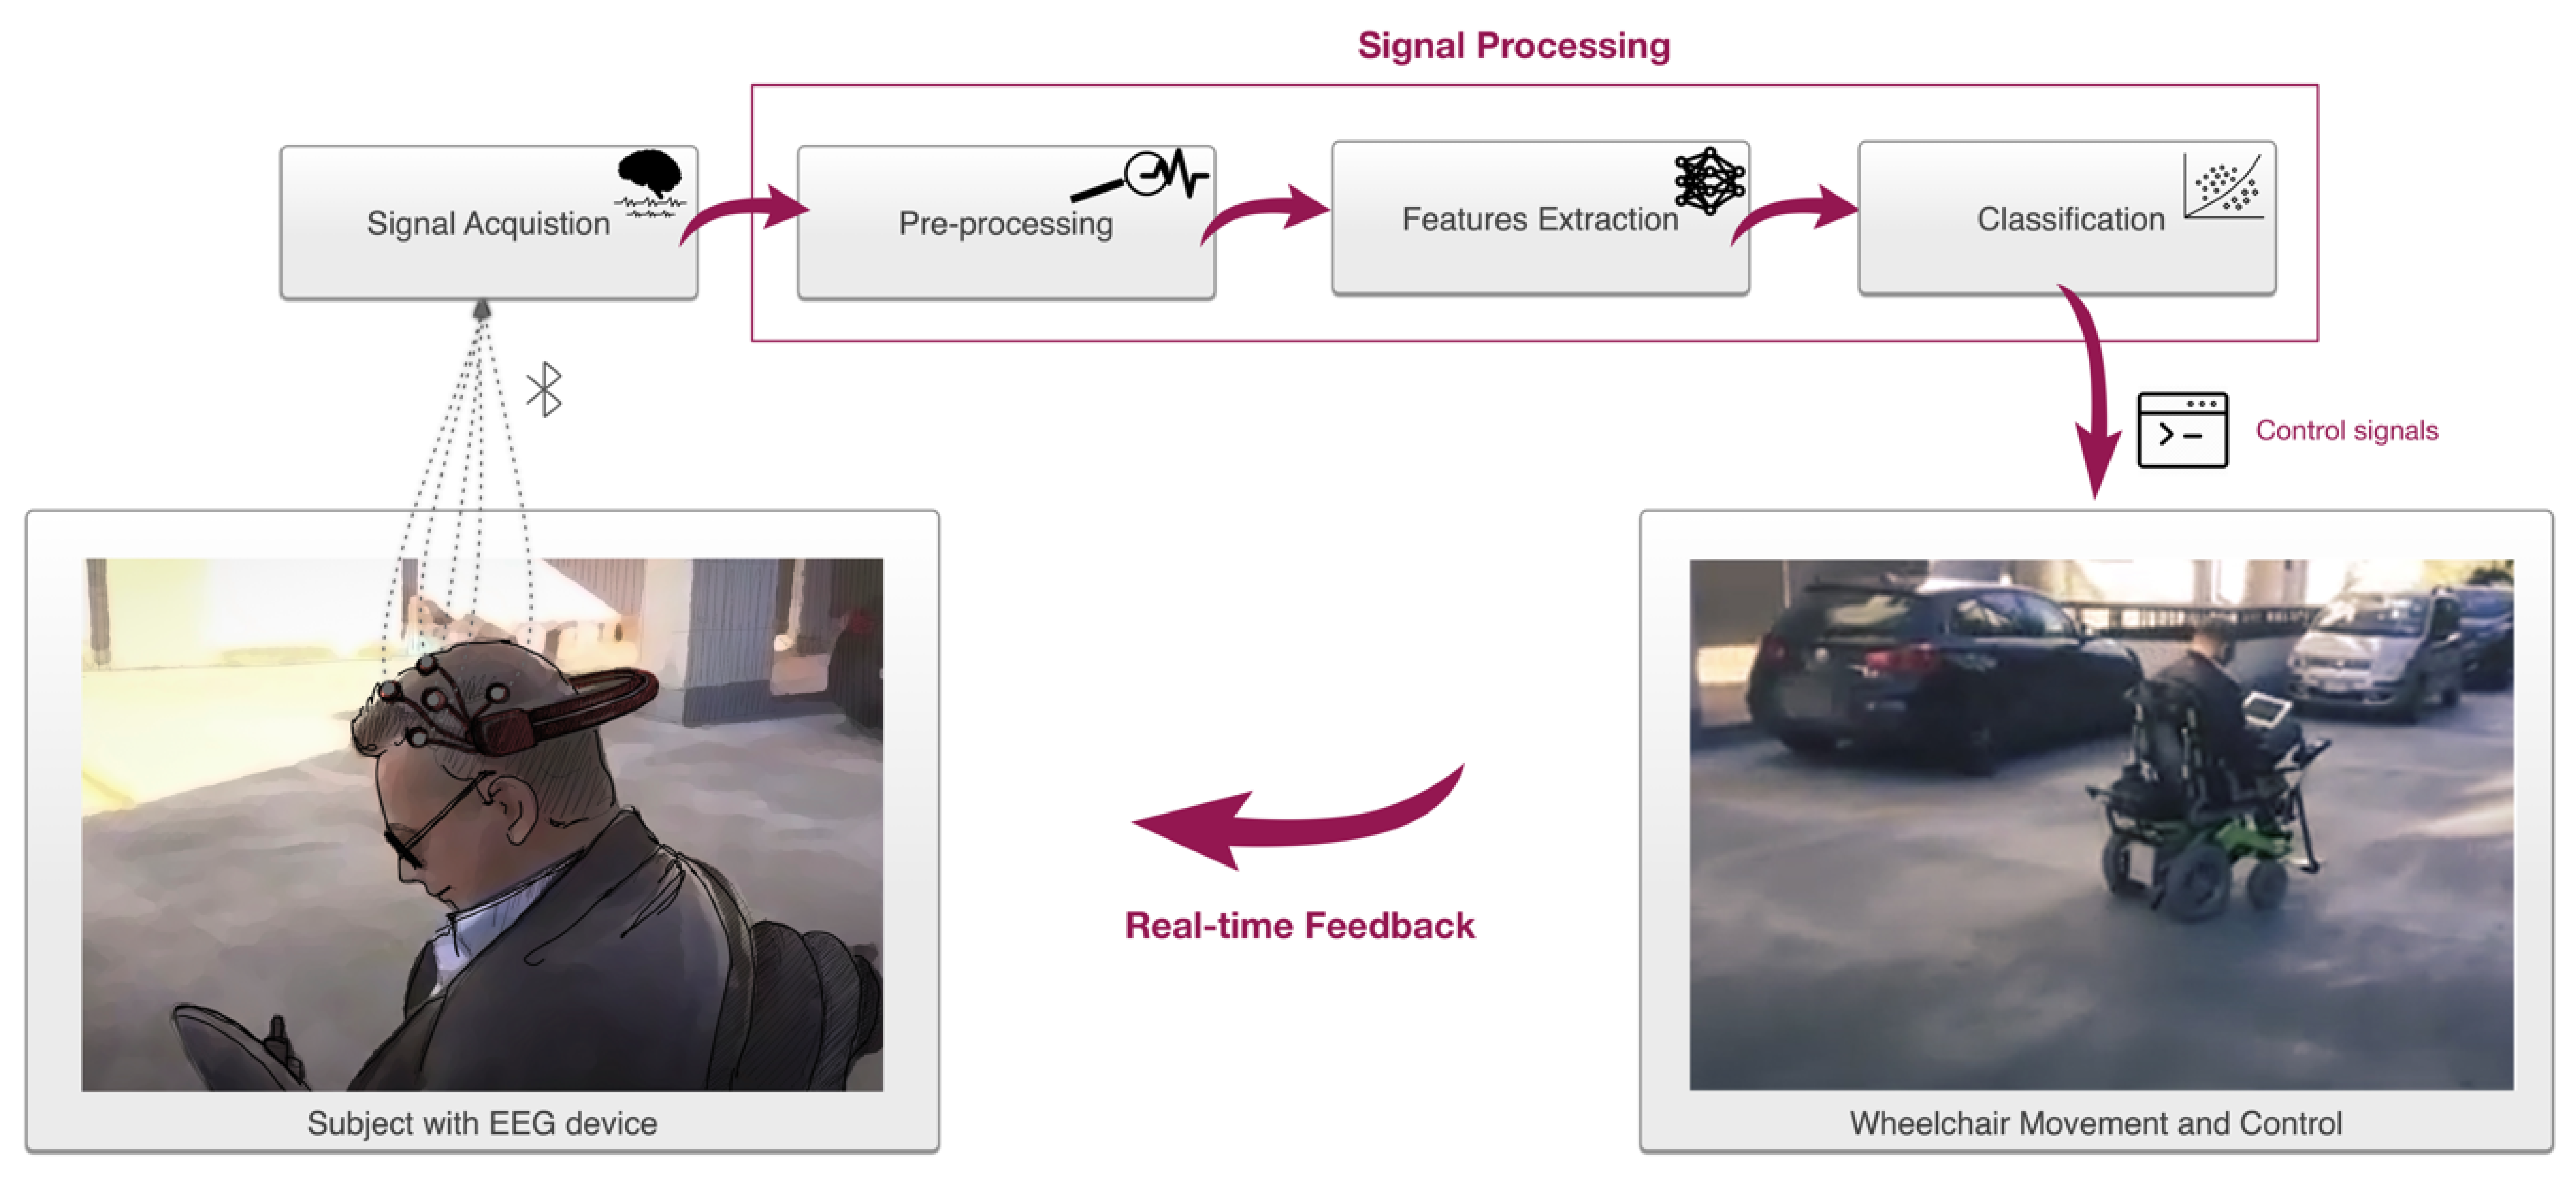
\includegraphics[width=0.4\textwidth]{figures/literature/realcase/wheelchair_control}
            };
            \node (page7) [yshift=0cm, xshift=-.5cm, rotate=30] {
                
\includegraphics[width=0.4\textwidth]{figures/literature/realcase/StrokeRehabilitation_paper}
            };
            \node (page8) [yshift=0cm, xshift=.5cm, rotate=-30] {
                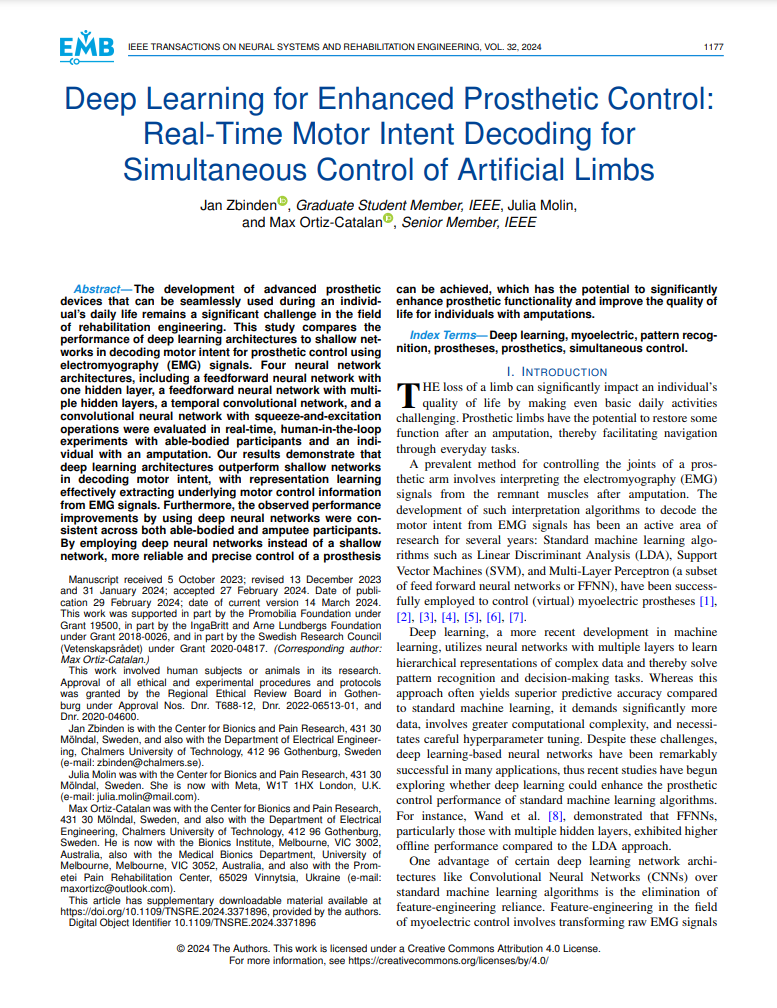
\includegraphics[width=0.4\textwidth]{figures/literature/realcase/ProsthesisControl_paper}
            };
            \node (page10) [yshift=0cm, xshift=0cm, rotate=0] {
                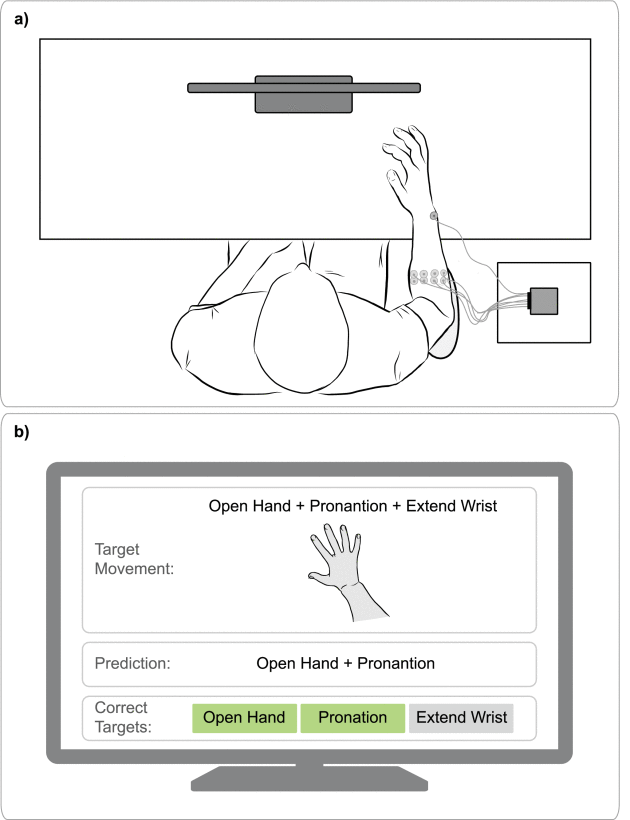
\includegraphics[width=0.4\textwidth]{figures/literature/realcase/limb_control}
            };
        \end{tikzpicture}
    \end{minipage}
\end{frame}

% \begin{frame}{Related Works~\textemdash{}~EEG MI Classifier}
%     \begin{minipage}[c]{0.65\textwidth}
%         \begin{itemize}
%             \item CNN-based approach
%             \item RNN-based approach
%             \item Transformer-based approach
%             \item Machine Learning-based approach
%         \end{itemize}
%     \end{minipage}
%     \begin{minipage}[c]{0.33\textwidth}
%         \vspace*{-.5cm}
%         \hspace*{-.7cm}
%         \begin{tikzpicture}
%             \node (page1) [xshift=-.7cm, rotate=30] {
%                 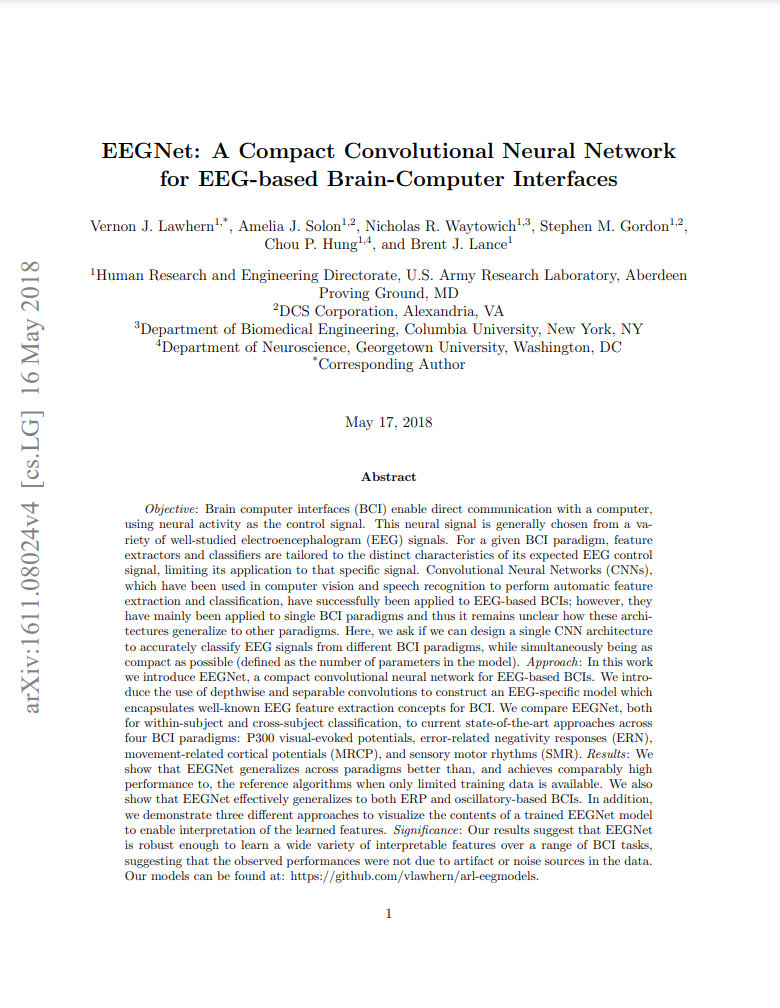
\includegraphics[width=0.6\textwidth]{figures/literature/classifier/EEGNet_paper}
%             };
%             \node (page2) [xshift=.7cm, rotate=-30] {
%                 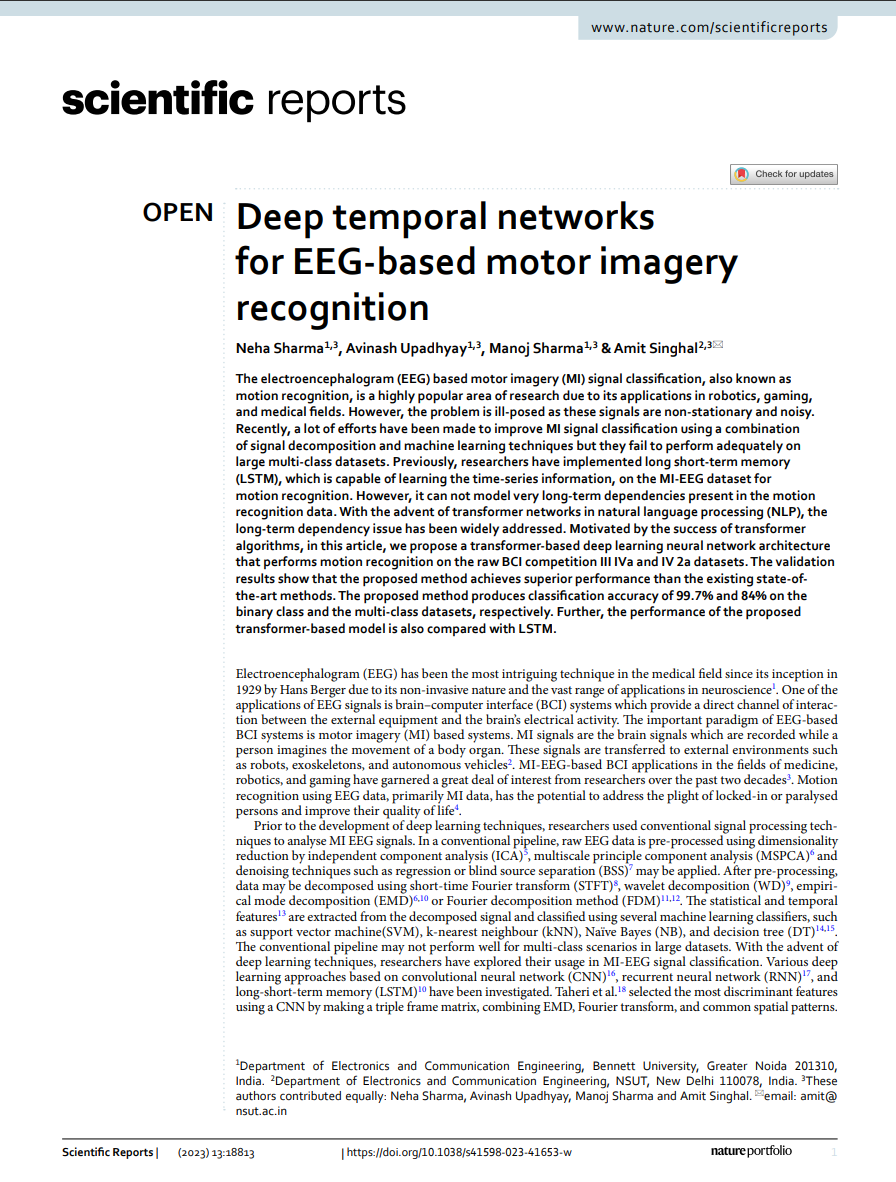
\includegraphics[width=0.6\textwidth]{figures/literature/classifier/LSTM_Transformer_paper}
%             };
%         \end{tikzpicture}
%     \end{minipage}
% \end{frame}
% \begin{frame}{Related Works~\textemdash{}~Dataset Augmentation}
%     \begin{minipage}[c]{0.65\textwidth}
%         \begin{itemize}
%             \item Generative Adversarial Networks (GANs)
%             \item Noise Injection
%             \item Random Sampling
%         \end{itemize}
%     \end{minipage}
%     \begin{minipage}[c]{0.33\textwidth}
%         \vspace*{-.5cm}
%         \hspace*{-.7cm}
%         \begin{tikzpicture}
%             \node (page3) [xshift=-.7cm, rotate=30] {
%                 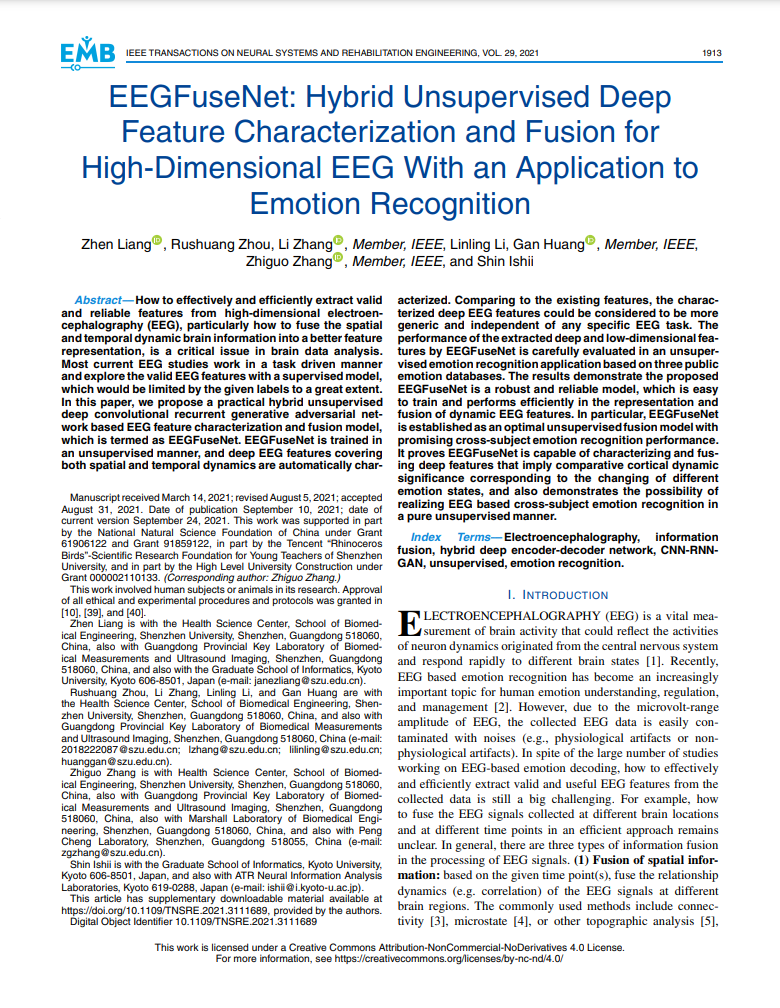
\includegraphics[width=0.6\textwidth]{figures/literature/augmentation/EEGFuseNet_paper}
%             };
%             \node (page4) [xshift=.7cm, rotate=-30] {
%                 
\includegraphics[width=0.6\textwidth]{figures/literature/augmentation/NoiseInjection_paper}
%             };
%         \end{tikzpicture}
%     \end{minipage}
% \end{frame}
% \begin{frame}{Related Works~\textemdash{}~User Game Feel and Experience}
%     \begin{minipage}[c]{0.65\textwidth}
%         \begin{itemize}
%             \item Engagement
%             \item Flow
%             \item Immersion
%             \item Presence
%         \end{itemize}
%     \end{minipage}
%     \begin{minipage}[c]{0.33\textwidth}
%         \vspace*{-.5cm}
%         \hspace*{-.7cm}
%         \begin{tikzpicture}
%             \node (page5) [xshift=-.7cm, rotate=30] {
%                 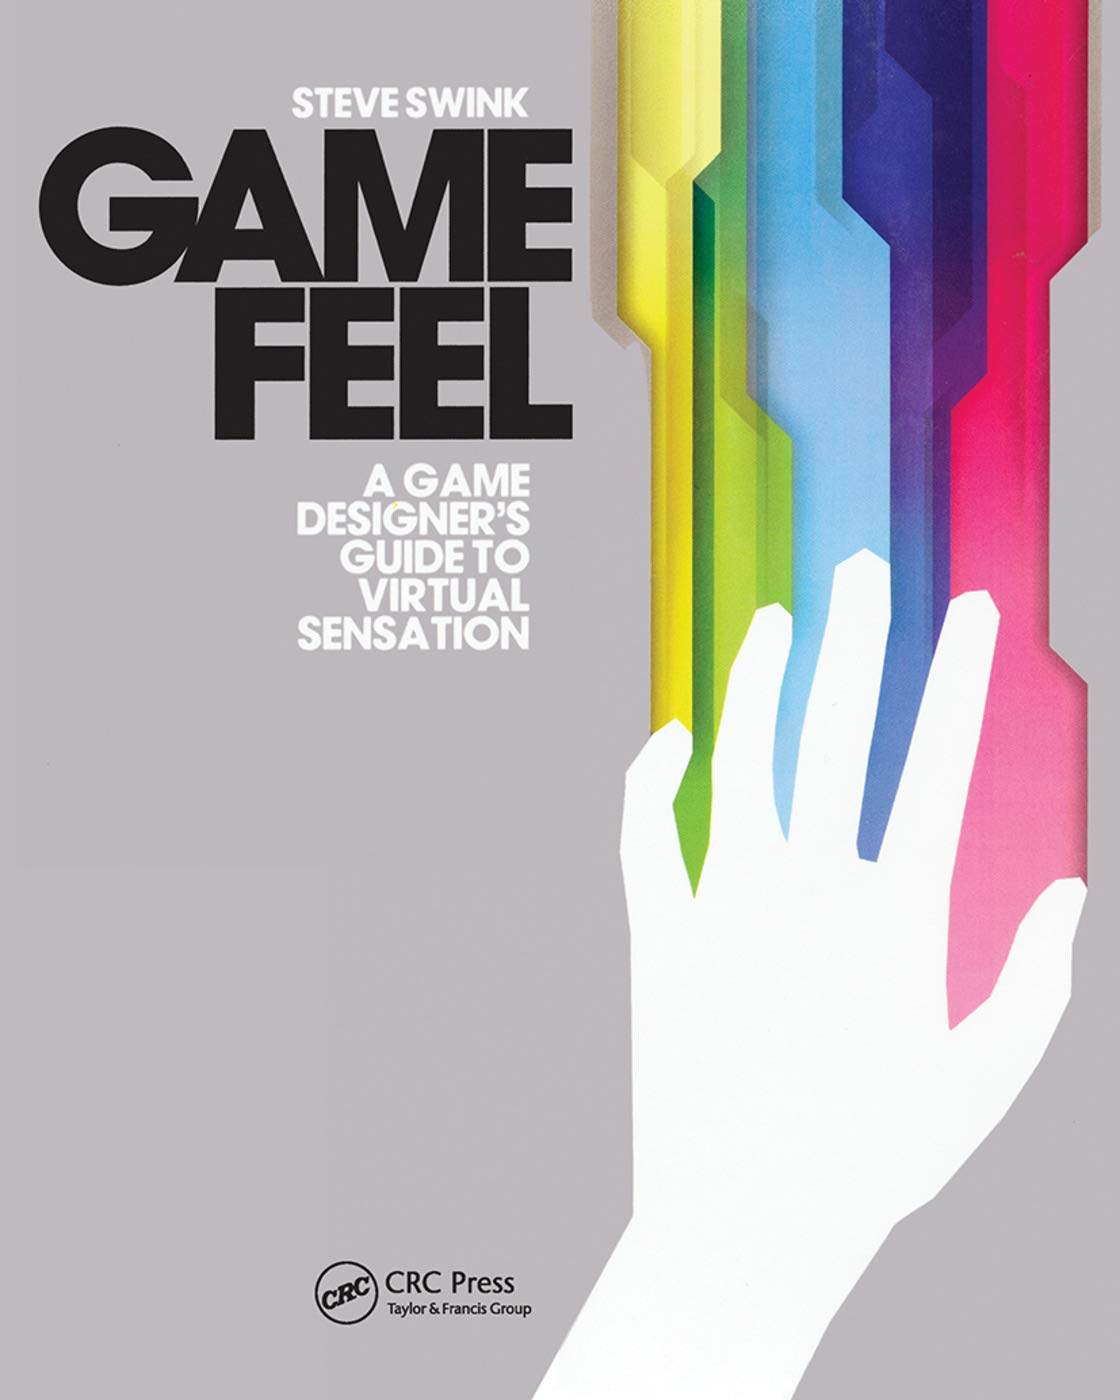
\includegraphics[width=0.6\textwidth]{figures/literature/gamefeel/GameFeel_book}
%             };
%             \node (page6) [xshift=.7cm, rotate=-30] {
%                 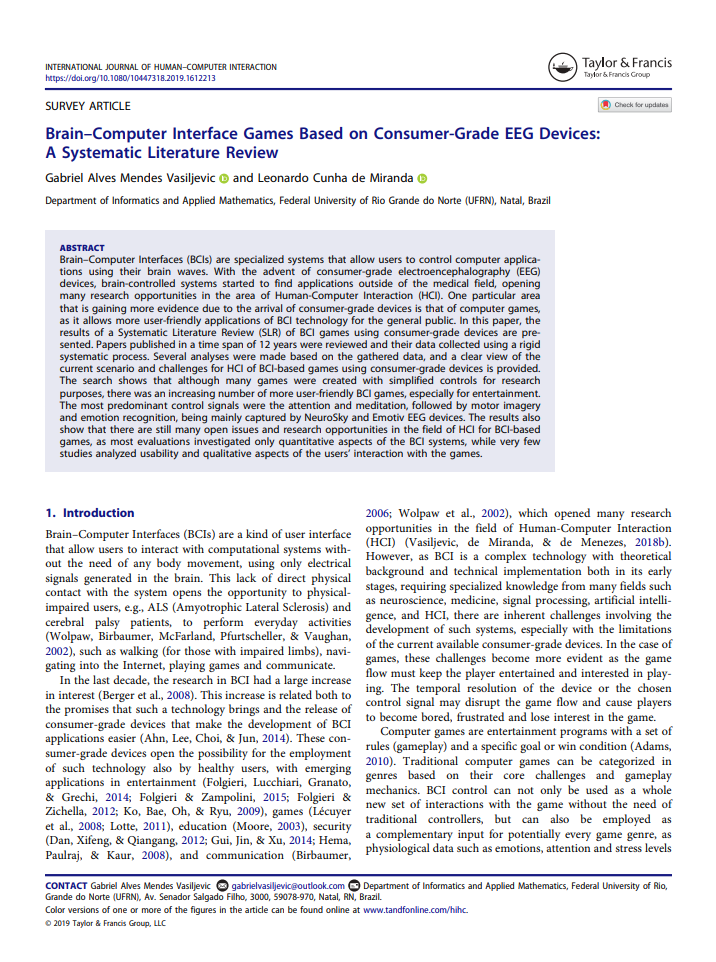
\includegraphics[width=0.6\textwidth]{figures/literature/gamefeel/BCI_Game_paper}
%             };
%         \end{tikzpicture}
%     \end{minipage}
% \end{frame}
% \begin{frame}{Related Works~\textemdash{}~EEG MI Uses in Real Case-Scenarios}
%     \begin{minipage}[c]{0.65\textwidth}
%         \begin{itemize}
%             \item Post-Stroke Rehabilitation
%             \item Prosthesis Control
%             \item Wheelchair Control
%         \end{itemize}
%     \end{minipage}
%     \begin{minipage}[c]{0.33\textwidth}
%         \vspace*{-.5cm}
%         \hspace*{-.7cm}
%         \begin{tikzpicture}
%             \node (page8) [yshift=1cm, xshift=-.75cm, rotate=30] {
%                 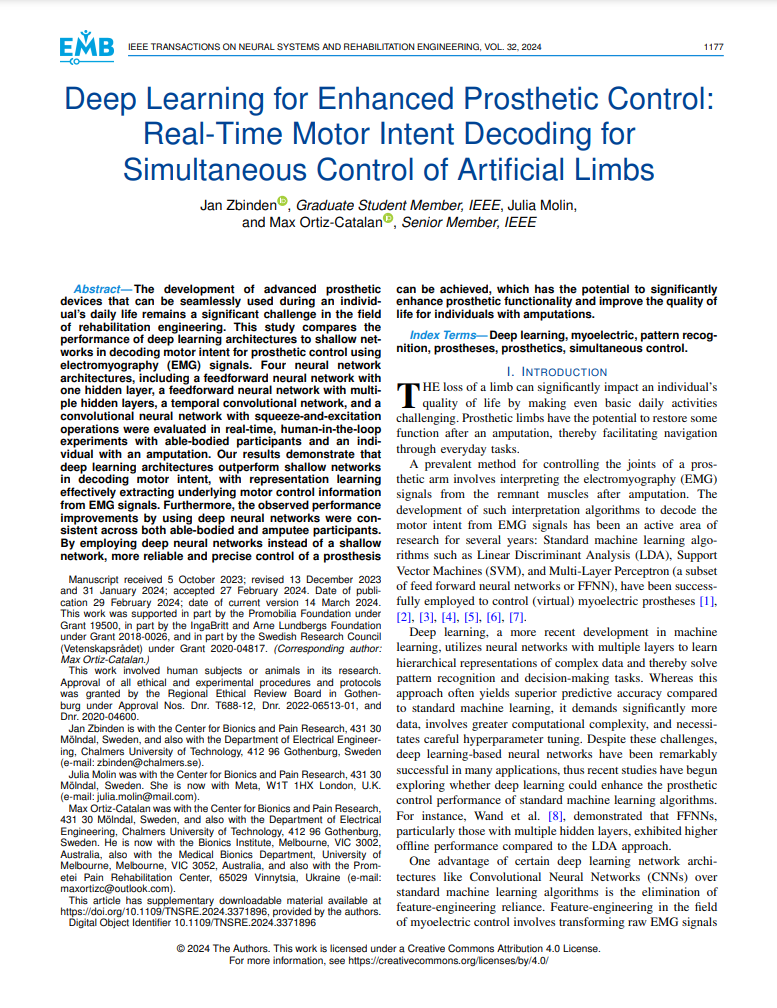
\includegraphics[width=0.65\textwidth]{figures/literature/realcase/ProsthesisControl_paper}
%             };
%             \node (page7) [yshift=1cm, xshift=.75cm, rotate=-30] {
%                 
\includegraphics[width=0.65\textwidth]{figures/literature/realcase/StrokeRehabilitation_paper}
%             };
%             \node (page10) [yshift=0cm, xshift=0cm, rotate=0] {
%                 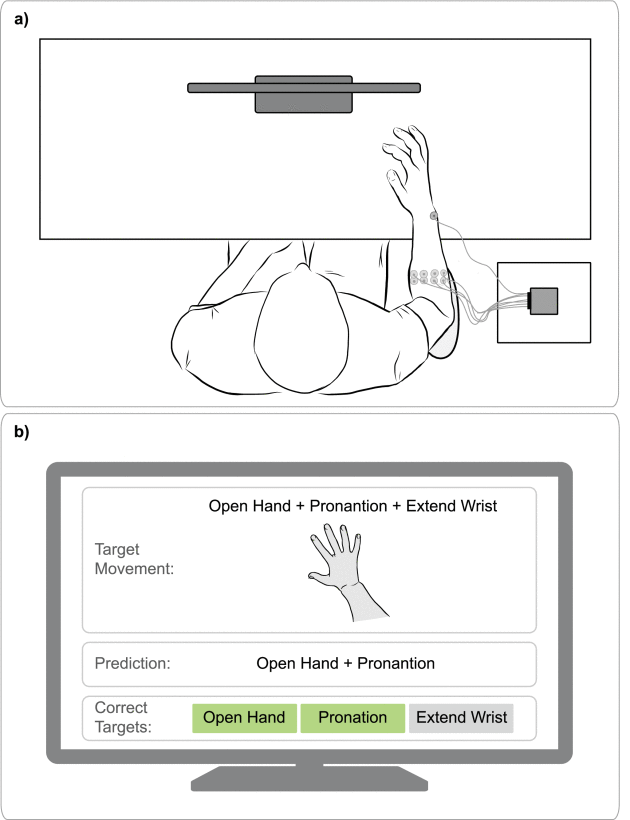
\includegraphics[width=0.65\textwidth]{figures/literature/realcase/limb_control}
%             };
%             \node (page9) [yshift=-1.5cm, xshift=.75cm, rotate=-30] {
%                 
\includegraphics[width=0.65\textwidth]{figures/literature/realcase/WheelchairControl_paper}
%             };
%             \node (page11) [yshift=-1.5cm, xshift=-.75cm, rotate=30] {
%                 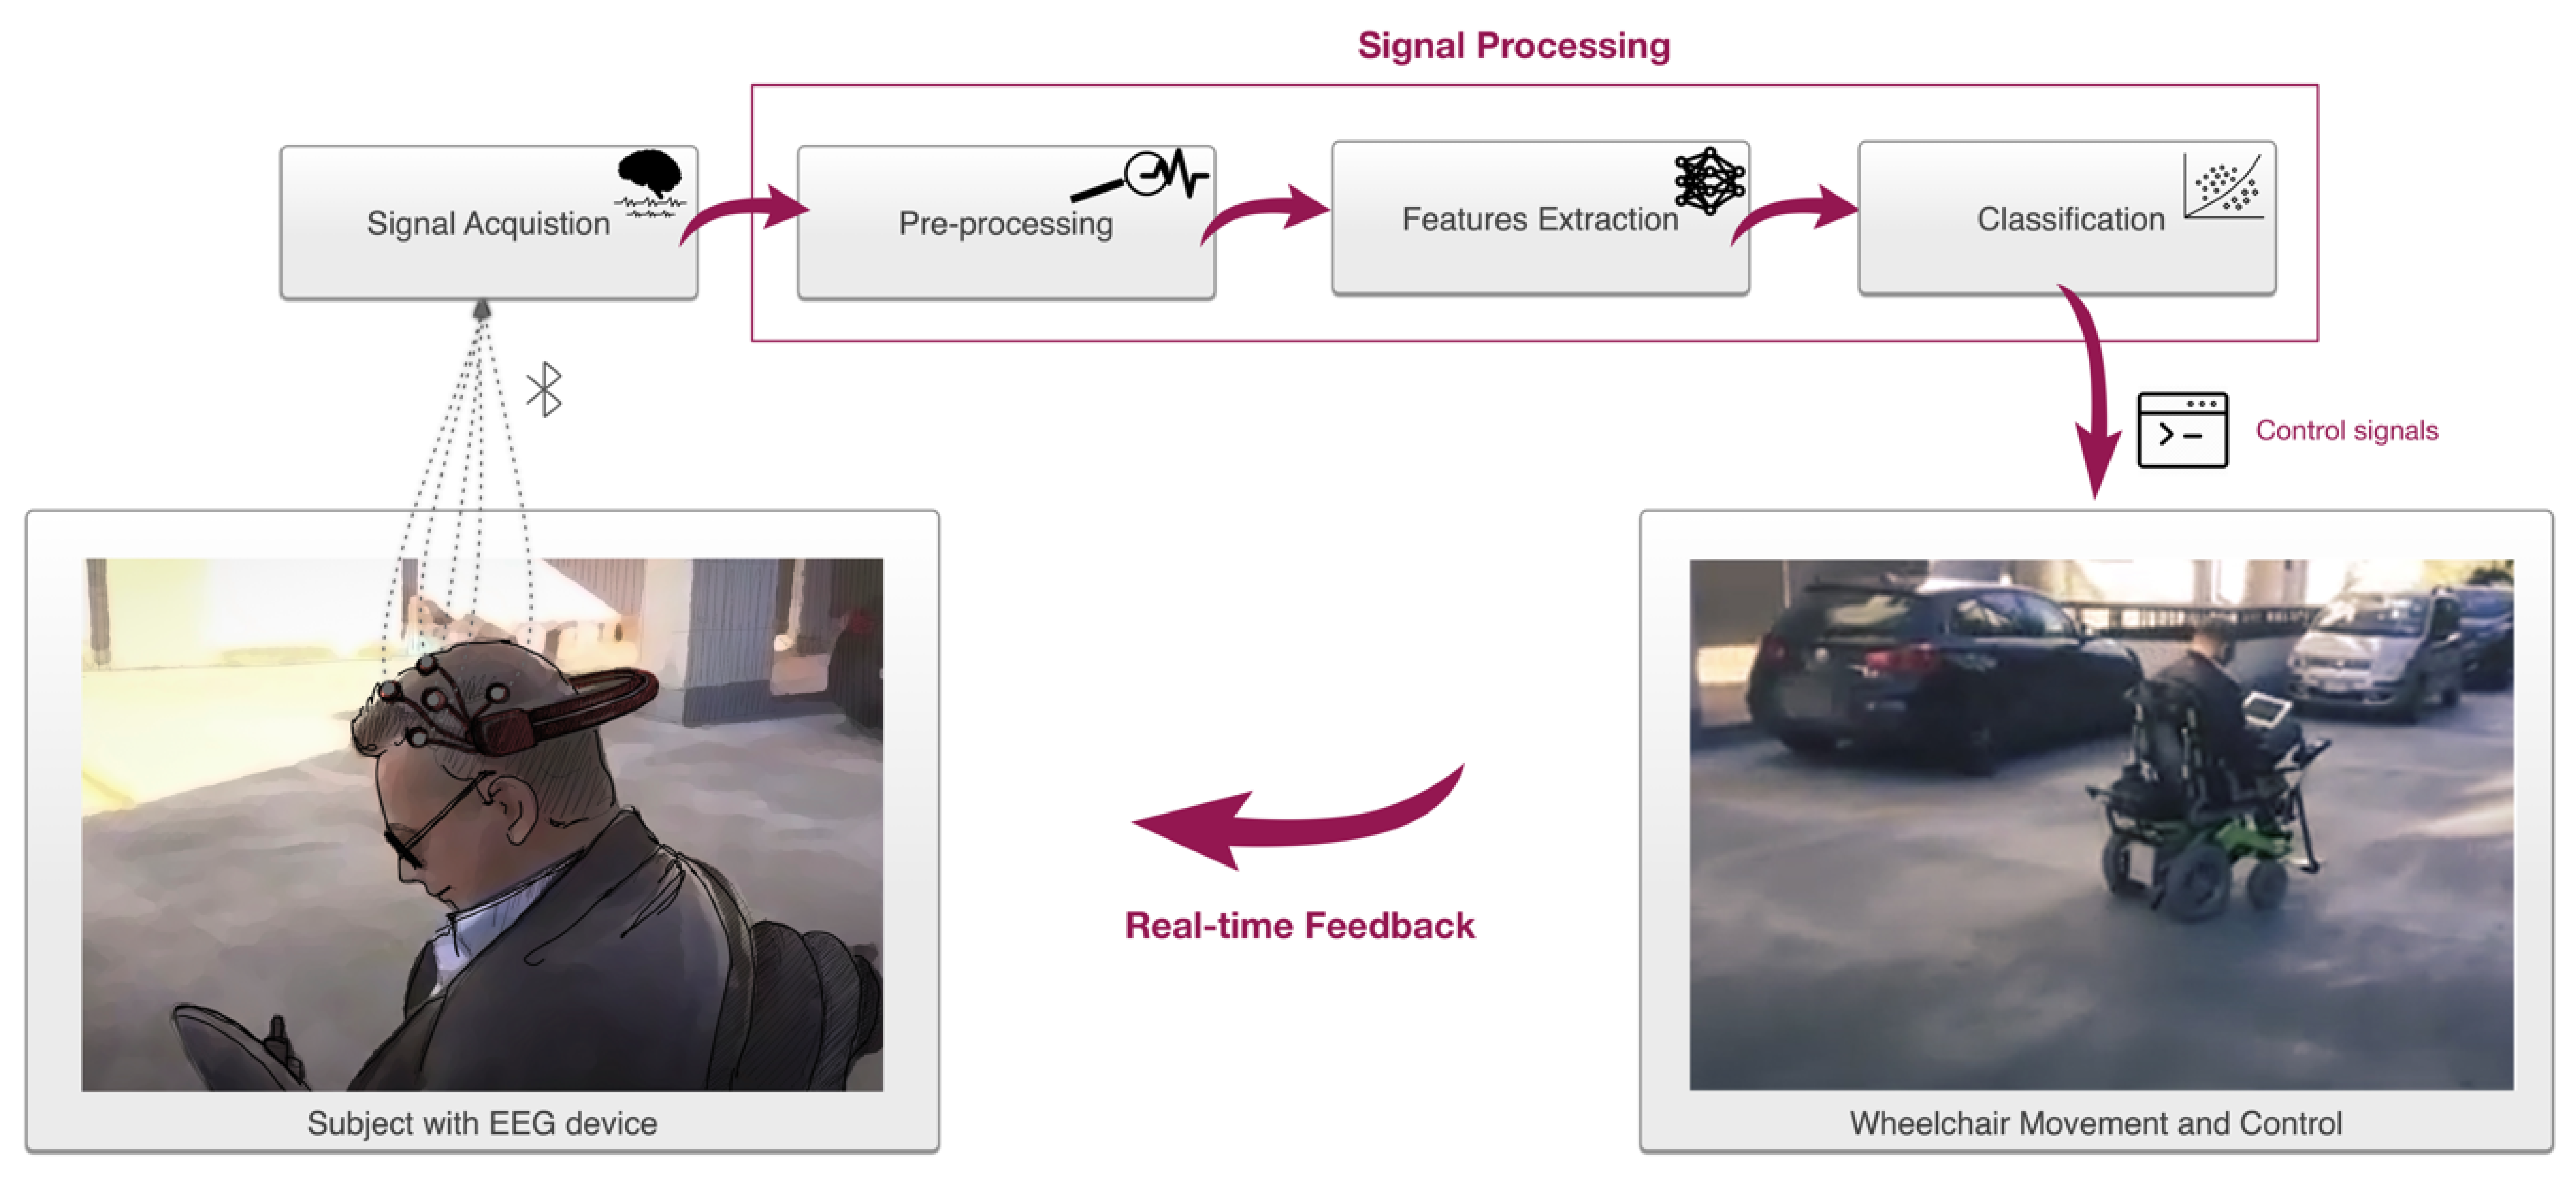
\includegraphics[width=0.65\textwidth]{figures/literature/realcase/wheelchair_control}
%             };
%         \end{tikzpicture}
%     \end{minipage}
% \end{frame}

\section{Development}
\begin{frame}{<title>}
\begin{center}
    
\end{center}
\end{frame}
\section{Results}
\begin{frame}{Results}
    \begin{itemize}
        \item Testing
        \item Human Study
    \end{itemize}
\end{frame}

\subsection*{Technical Performance Mesurement}
\begin{frame}{Technical Performance Mesurement}
    \begin{itemize}
        \item Classification Accuracy
        \item Latency
        \item Robustness
        \item Other Metrics
    \end{itemize}
\end{frame}

\begin{frame}{TPM \textemdash{} Classification Accuracy}

\begin{table}[!htbp]
    \centering
    \begin{tabular}{|c||c|c|c|c|}
        \hline
        & \textbf{Feet} & \textbf{Left Hand} & \textbf{Right Hand} & \textbf{Rest} \\
        \hline
        \hline
        \textbf{Feet} & \textbf{779} & 367 & 259 & 314 \\
        \hline
        \textbf{Left Hand} & 284 & \textbf{1005} & 189 & 258 \\
        \hline
        \textbf{Right Hand} & 356 & 243 & \textbf{840} & 268 \\
        \hline
        \textbf{Rest} & 1474 & 1188 & 1158 & \textbf{3067} \\
        \hline
    \end{tabular}
    \caption{Confusion matrix of the validation dataset. \textbf{47.23\%} Accuracy}
\end{table}
\begin{table}[!htbp]
    \centering
    \begin{tabular}{|c||c|c|c|c|}
        \hline
        & \textbf{Feet} & \textbf{Left Hand} & \textbf{Right Hand} & \textbf{Rest} \\
        \hline
        \hline
        \textbf{Feet} & \textbf{824} & 104 & 38 & 34 \\
        \hline
        \textbf{Left Hand} & 16 & \textbf{961} & 1 & 22 \\
        \hline
        \textbf{Right Hand} & 28 & 51 & \textbf{789} & 132 \\
        \hline
        \textbf{Rest} & 1 & 6 & 1 & \textbf{992} \\
        \hline
    \end{tabular}
    \caption{Confusion matrix of the GAN data. \textbf{89.15\%} Accuracy}
\end{table}

\end{frame}
\begin{frame}{TPM \textemdash{} Latency}
    \begin{figure}[!htbp]
        \scalebox{1}[1]{
        \begin{tikzpicture}
            % Horizontal line
            \draw[thick] (0,0) -- (7.6625,0);
            \draw[thick, dashed] (7.6625,0) -- (8.15,0);
            \draw[thick, -Triangle] (8.15,0) -- (10,0) node[font=\scriptsize,below left=3pt and -8pt]{\textbf{ms}};
            % \draw[thick, dashed] (9,0) -- (9.5,0);
            % \draw[thick, -Triangle] (9,0) -- (10,0) node[font=\scriptsize,below left=3pt and -8pt]{\textbf{ms}};
    
            % Start of the timeline
            \draw (0,-0.1) -- (0,0.1) node[font=\scriptsize,below left=3pt and -6pt]{\textbf{0}};
            \node[font=\scriptsize,left=3pt] at (0,0) [anchor=east]{\textbf{Min}};
    
            % Image Processing Time
            \draw (0.1625, -0.1) -- (0.1625, 0.1) node[font=\scriptsize,below left=3pt and -10pt]{\textbf{\textcolor{olive}{13}}};
            \fill[purple] (0, 0.2) rectangle (0.1625, 0.4);
            
            % \draw (1, -0.1) -- (1, 0.1) node[font=\scriptsize,below left=3pt and -8pt]{\textbf{\textcolor{red}{80}}};
            % \fill[purple] (0,-0.4) rectangle (1,-0.6);
            
            % Motor Response Time
            \draw (1.4125, -0.1) -- (1.4125, 0.1) node[font=\scriptsize,below left=3pt and -10pt]{\textbf{\textcolor{olive}{113}}};
            \fill[blue] (0.1625, 0.4) rectangle (1.4125, 0.6);
    
            % \draw (2.75, -0.1) -- (2.75, 0.1) node[font=\scriptsize,below left=3pt and -10pt]{\textbf{\textcolor{red}{220}}};
            % \fill[blue] (1,-0.6) rectangle (2.75,-0.8);
    
            % Motor Response Recording Time
            \draw (7.6625, -0.1) -- (7.6625, 0.1) node[font=\scriptsize,below left=3pt and -8pt]{\textbf{\textcolor{olive}{613}}};
            \fill[red] (1.4125, 0.6) rectangle (7.6625, 0.8);
    
            % \draw (9, -0.1) -- (9, 0.1) node[font=\scriptsize,below left=3pt and -10pt]{\textbf{\textcolor{red}{720}}};
            % \fill[red] (2.75,-0.8) rectangle (9,-1);
    
            % Signal Classification Time
            \draw (8.15, -0.1) -- (8.15, 0.1) node[font=\scriptsize,below left=3pt and -10pt]{\textbf{\textcolor{olive}{615}}};
            \fill[amethyst] (7.6625, 0.8) rectangle (8.15, 1);
    
            % \draw (9.5, -0.1) -- (9.5, 0.1) node[font=\scriptsize,below left=3pt and -10pt]{\textbf{\textcolor{red}{732}}};
            % \fill[amethyst] (9,-1) rectangle (9.5,-1.2);
    
            % diff curly brace
            % \draw [decorate,decoration={brace,amplitude=5pt}] (8.15, 1) -- (9.5,1) node [anchor=south,midway,above=4pt] {\footnotesize Signal Received by Application};
        \end{tikzpicture}
        }
        \scalebox{1}[1]{
        \begin{tikzpicture}
                % Horizontal line
                \draw[thick] (0,0) -- (9,0);
                % \draw[thick, dashed] (7.6625,0) -- (8.15,0);
                % \draw[thick] (8.15,0) -- (9,0);
                \draw[thick, dashed] (9,0) -- (9.5,0);
                \draw[thick, -Triangle] (9.5,0) -- (10,0) node[font=\scriptsize,below left=3pt and -8pt]{\textbf{ms}};
    
                % Start of the timeline
                \draw (0,-0.1) -- (0,0.1) node[font=\scriptsize,below left=3pt and -6pt]{\textbf{0}};
                \node[font=\scriptsize,left=3pt] at (0,0) [anchor=east]{\textbf{Max}};
    
                % Image Processing Time
                % \draw (0.1625, -0.1) -- (0.1625, 0.1) node[font=\scriptsize,below left=3pt and -10pt]{\textbf{\textcolor{olive}{13}}};
                % \fill[purple] (0, 0.2) rectangle (0.1625, 0.4);
                
                \draw (1, -0.1) -- (1, 0.1) node[font=\scriptsize,below left=3pt and -8pt]{\textbf{\textcolor{red}{80}}};
                \fill[purple] (0,0.2) rectangle (1,0.4);
                
                % Motor Response Time
                % \draw (1.4125, -0.1) -- (1.4125, 0.1) node[font=\scriptsize,below left=3pt and -10pt]{\textbf{\textcolor{olive}{113}}};
                % \fill[blue] (0.1625, 0.4) rectangle (1.4125, 0.6);
    
                \draw (2.75, -0.1) -- (2.75, 0.1) node[font=\scriptsize,below left=3pt and -10pt]{\textbf{\textcolor{red}{220}}};
                \fill[blue] (1,0.4) rectangle (2.75,0.6);
    
                % Motor Response Recording Time
                % \draw (7.6625, -0.1) -- (7.6625, 0.1) node[font=\scriptsize,below left=3pt and -8pt]{\textbf{\textcolor{olive}{613}}};
                % \fill[red] (1.4125, 0.6) rectangle (7.6625, 0.8);
    
                \draw (9, -0.1) -- (9, 0.1) node[font=\scriptsize,below left=3pt and -10pt]{\textbf{\textcolor{red}{720}}};
                \fill[red] (2.75,0.6) rectangle (9,0.8);
    
                % Signal Classification Time
                % \draw (8.15, -0.1) -- (8.15, 0.1) node[font=\scriptsize,below left=3pt and -10pt]{\textbf{\textcolor{olive}{614}}};
                % \fill[amethyst] (7.6625, 0.8) rectangle (8.15, 1);
    
                \draw (9.5, -0.1) -- (9.5, 0.1) node[font=\scriptsize,below left=3pt and -10pt]{\textbf{\textcolor{red}{745}}};
                \fill[amethyst] (9,0.8) rectangle (9.5,1);
    
                % diff curly brace
                % \draw [decorate,decoration={brace,amplitude=5pt}] (8.15, 1) -- (9.5,1) node [anchor=south,midway,above=4pt] {\footnotesize Signal Received by Application};    
        \end{tikzpicture}
        }
        \begin{itemize}
            \item \textcolor{purple}{Brain Processing Image Time:} 13-80 ms
            \item \textcolor{blue}{Brain Motor Response Activation Time:} 100-140 ms
            \item \textcolor{red}{BCI Motor Response Recording Time:} 500 ms
            \item \textcolor{amethyst}{Signal Classification Time:} 1.10-24.67 ms
        \end{itemize}
        \caption{Latency of the system in a real case scenario.}\label{fig:latency}
    \end{figure}
\end{frame}
\begin{frame}{TPM \textemdash{} Robustness}
    \begin{figure}[!htbp]
        \centering
        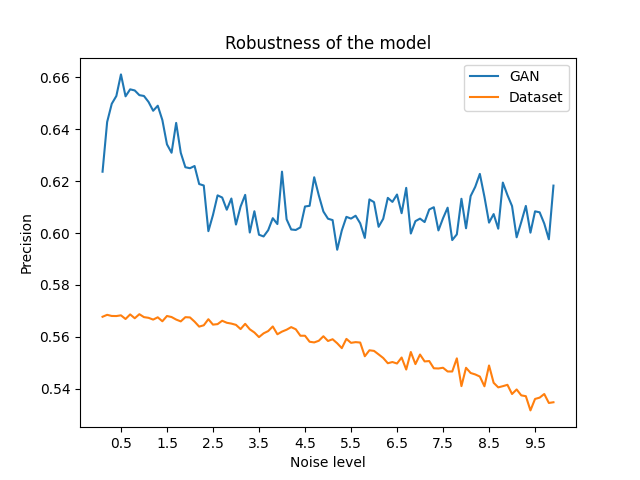
\includegraphics[width=0.8\textwidth]{figures/Testing/robustness_plot}
        \caption{Robustness of the system in case of noise in the data.}\label{fig:robustness}
    \end{figure}
\end{frame}
\begin{frame}{TPM \textemdash{} Other Metrics}
    \begin{itemize}
        \item Portability: Written in Python with Torch for CUDA
        \item Efficiency: Can run on most modern Hardware Platforms
        \item Maintainability: 6.55 PyLint Score
    \end{itemize}
    \begin{table}[!htbp]
        \centering
        \scalebox{.8}{
        \begin{tabular}{|c||c|c|c|}
            \hline
            \textbf{Resource} & \textbf{Minimum Usage} & \textbf{Average Usage} & \textbf{Maximum Usage} \\
            \hline
            \hline
            K-FLOPS & 754 & 754 & 754\\
            \hline
            CPU Memory & 30 KB & 47 KB & 90 KB \\
            \hline
            GPU CUDA Memory & 277 KB & 17.7 MB  & 41.3 MB \\
            \hline
        \end{tabular}
        }
        \caption{Efficiency of the system in terms of resource usage.}
    \end{table}
\end{frame}

\subsection*{Human Study}
\begin{frame}{Human Study}
    \begin{itemize}
        \item Study Design
        \item Participants
        \item Procedure
        \item Game Design
        \item Data Collection
        \item User Experience Survey
        \item Pre-Testing
    \end{itemize}
\end{frame}
\begin{frame}{Human Study \textemdash{} Study Design}
    \begin{itemize}
        \item Play Video Game with EEG Headset and Motor Imagery
        \item Controlled Environment
        \item User Experience Survey
    \end{itemize}
\end{frame}
\begin{frame}{Human Study \textemdash{} Participants}
    \begin{itemize}
        \item Healthy Adults
        \item No History of Neurological Disorders
        \item Informed Participation
    \end{itemize}
\end{frame}
\begin{frame}{Human Study \textemdash{} Procedure}
    \begin{itemize}
        \item Play Game for Predetermined Time
        \item Fill Out User Experience Survey
        \item Single Session
        \item Flexible Environment 
    \end{itemize}
\end{frame}
\begin{frame}{Human Study \textemdash{} Game Design}
    \begin{itemize}
        \item Engaging Game
        \item Simple Controls
    \end{itemize}
\end{frame}
\begin{frame}{Human Study \textemdash{} Data Collection}
    \begin{itemize}
        \item Screen Recording with Microphone
        \item Multiple Data Collection Points
        \item Identify System Issues
        \item Identify Improvement Areas
    \end{itemize}
\end{frame}
\begin{frame}{Human Study \textemdash{} User Experience Survey}
    \begin{itemize}
        \item Likert Scale (from 1 to 10)
        \item Included System Usability Scale (SUS)
        \item Included Game Experience Questionnaire
        \item Concise and Easy to Understand
    \end{itemize}
\end{frame}
\begin{frame}{Human Study \textemdash{} Pre-Testing}
    \begin{itemize}
        \item Verify the System Usability
        \item Verify Real-Time Data Collection
        \item Verify Lag and Delays
        \item Search Points of Failure
        \item Identified need for Fine Tuning
    \end{itemize}
\end{frame}


\section{Future Works}
\begin{frame}{Future Works}
\begin{itemize}
    \item Document and Clean the Code
    \item Improve or Change the Classification Algorithm
    \item Test different Classification Algorithms
    \item Perform Human Study
    \item Increase the number of Classification labels
\end{itemize}
\end{frame}
%%%%%%%%%%%%%%%%%%%%%%%%%%%%%%%%%%%%%%%%%%%%%%%%%%%%%%
%%%%%%%%%%%%%%%%%%%%%%%%%%%%%%%%%%%%%%%%%%%%%%%%%%%%%%
\section{\scshape}
\begin{frame}{}
\begin{center}
    
\includegraphics[width=6.5cm]{figures/thanks}
\end{center}
\end{frame}
%%%%%%%%%%%%%%%%%%%%%%%%%%%%%%%%%%%%%%%%%%%%%%%%%%%%%%
%%%%%%%%%%%%%%%%%%%%%%%%%%%%%%%%%%%%%%%%%%%%%%%%%%%%%%
\end{document}
